\chapter{Diseño e implementación del sistema}
Este capítulo describe la arquitectura general del sistema y detalla cada uno de sus componentes, desde el montaje electrónico del CanSat hasta la visualización de los datos en tiempo real.

Se justifica la elección del hardware y software empleados, se explica el funcionamiento del código embebido, y se documenta la integración entre los distintos módulos del sistema: la Raspberry Pi, el backend en Spring Boot, la base de datos, el broker de eventos RabbitMQ y el frontend desarrollado en Flutter.

Finalmente, se presentan las pruebas realizadas para verificar el funcionamiento del sistema completo.


\section{Selección de componentes y tecnologías utilizadas}


Este apartado describe los principales elementos hardware y software empleados en el sistema.

La selección se ha basado en los requisitos técnicos del proyecto y en las conclusiones del análisis comparativo desarrollado en el capítulo anterior.

\begin{itemize}
    \item \textbf{Unidad de procesamiento:} se ha utilizado una~\cite{raspberrypi_zero2}.

    \begin{figure}[H]
        \centering
        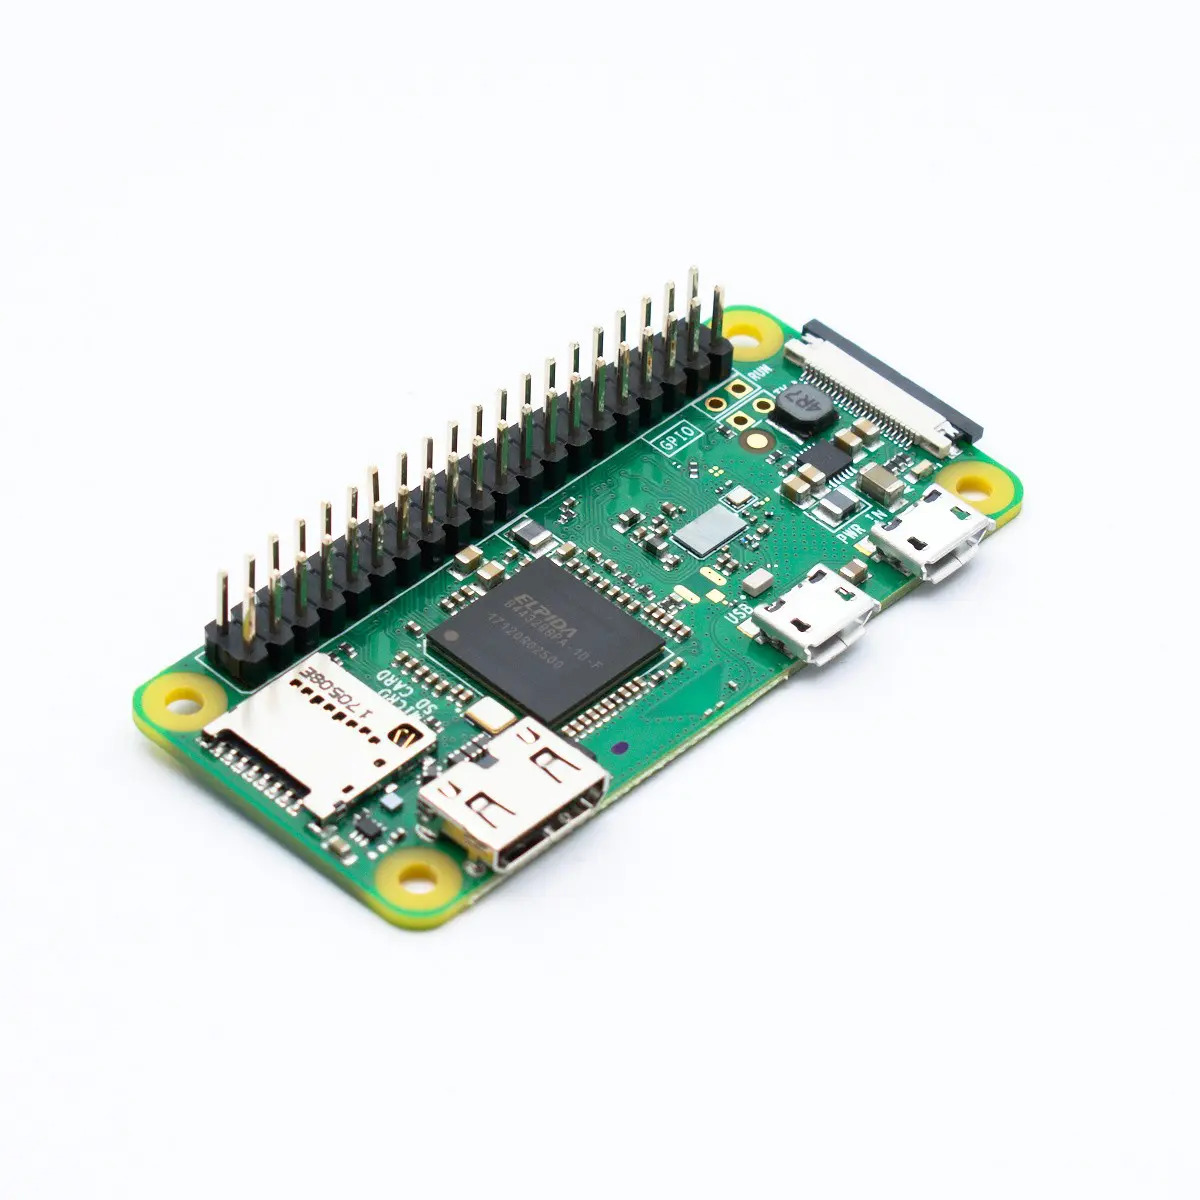
\includegraphics[width=0.2\textwidth]{Imagenes/Bitmap/ras2}
        \caption{Raspberry Pi Zero 2 W}
        \label{fig:ras2}
    \end{figure}

    Su capacidad para ejecutar Linux, capturar y codificar vídeo por hardware, y gestionar interfaces como I\textsuperscript{2}C, UART y CSI, la hacen adecuada para su integración directa en un CanSat sin necesidad de microcontroladores adicionales.
    \item \textbf{Sensor de presión barométrica:} el BMP388~\cite{adafruitBMP388} permite estimar la altitud mediante medición barométrica.
    Además de la presión atmosférica, proporciona la temperatura del entorno.
    Ofrece una precisión de ±8~Pa, bajo consumo y comunicación por I\textsuperscript{2}C.

    \begin{figure}[H]
        \centering
        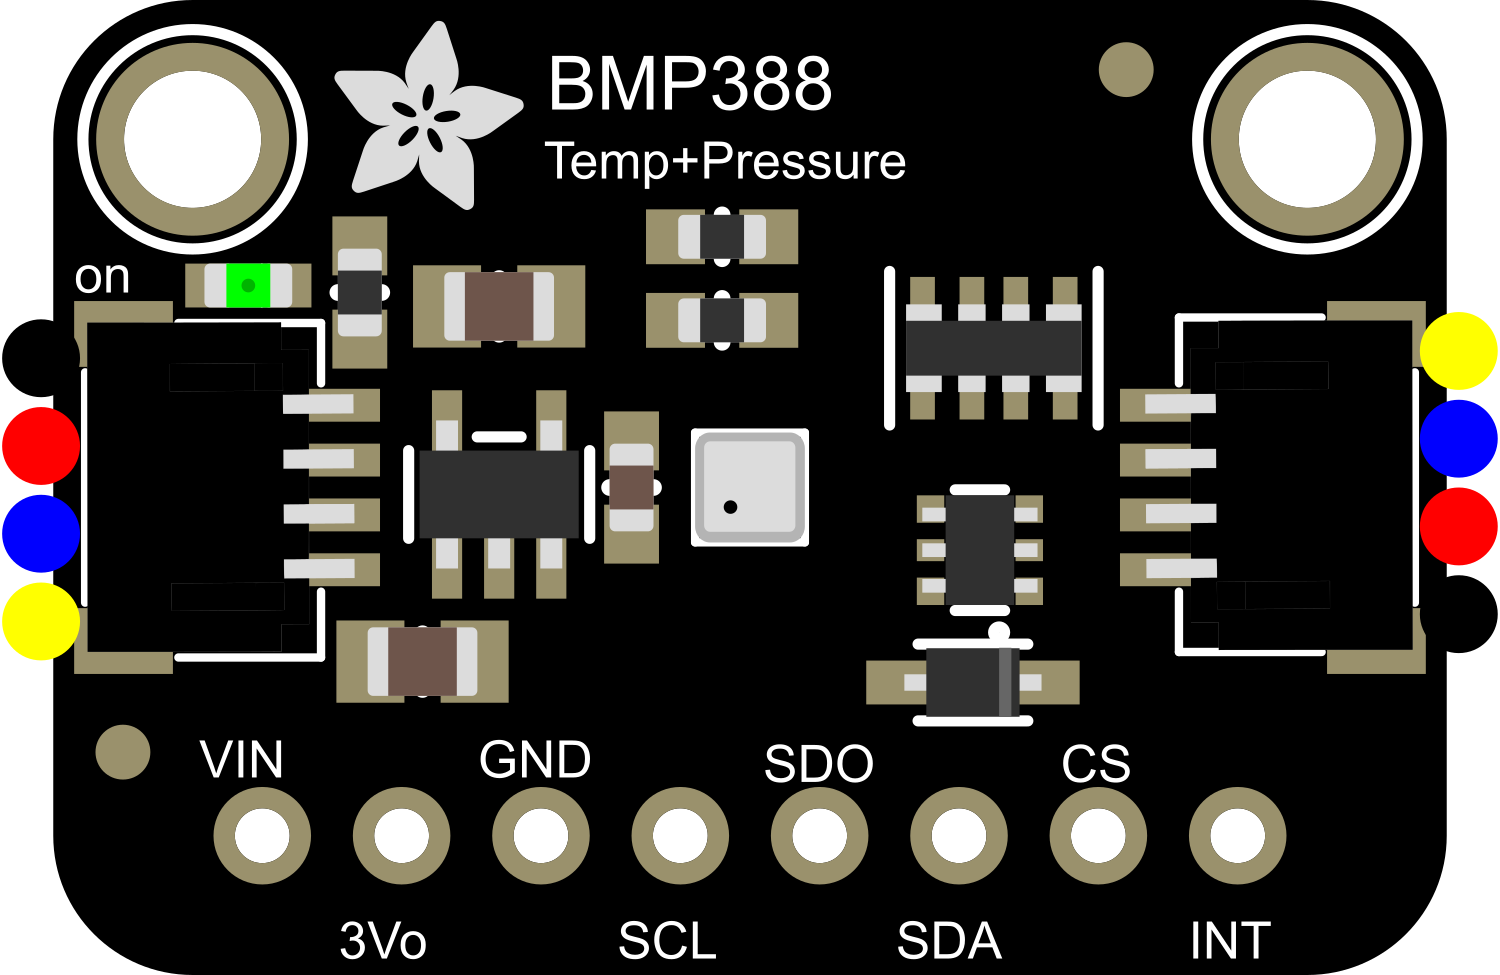
\includegraphics[width=0.4\textwidth]{Imagenes/Bitmap/bmp388}
        \caption{Sensor de presión barométrica bmp388}
        \label{fig:bmp388}
    \end{figure}

    \item \textbf{IMU:} Se ha empleado el BNO085~\cite{adafruitBNO085}, un sensor de 9 grados de libertad que combina acelerómetro, giroscopio y magnetómetro.
    Incorpora un procesador dedicado que realiza la fusión sensorial internamente y entrega directamente la orientación absoluta, lo que evita cálculos adicionales en la Raspberry Pi.

    \begin{figure}[H]
        \centering
        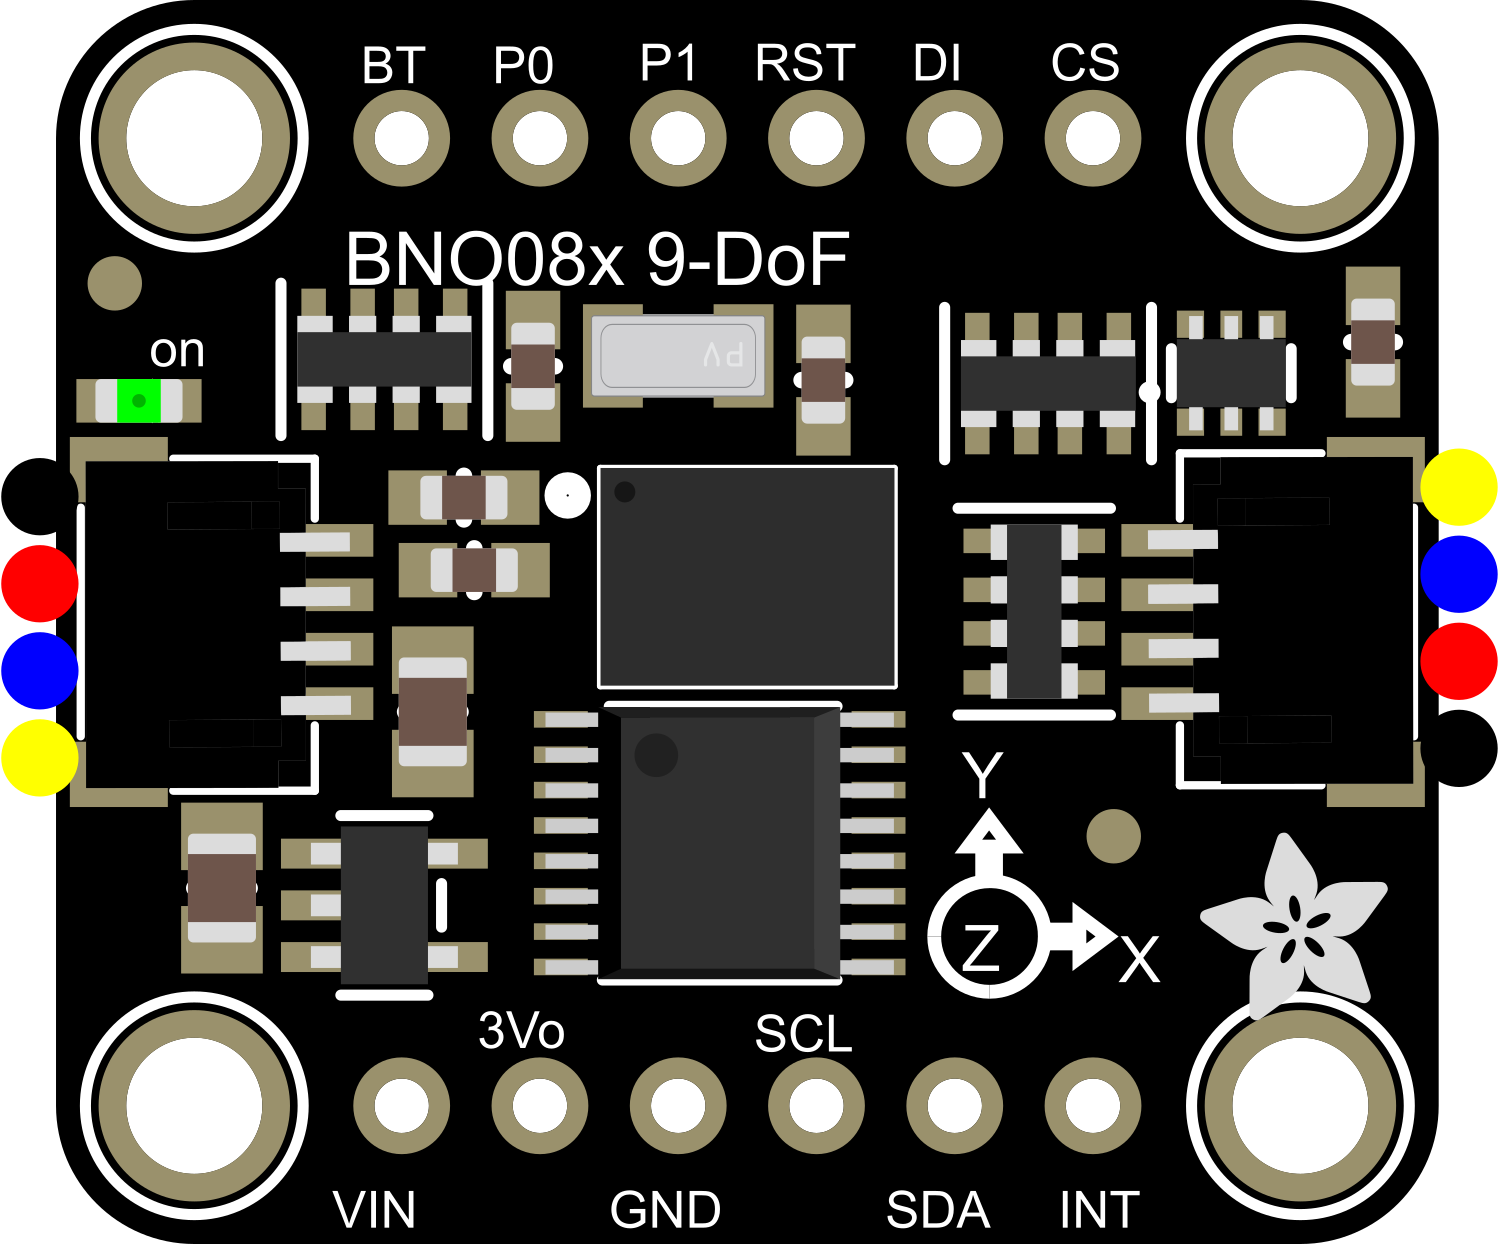
\includegraphics[width=0.4\textwidth]{Imagenes/Bitmap/bno085}
        \caption{IMU bno085}
        \label{fig:bno085}
    \end{figure}
    \item \textbf{GNSS:} se ha utilizado el módulo BN-880~\cite{bn880Module}, que integra un receptor GNSS con soporte para múltiples constelaciones (GPS, GLONASS, Galileo y BeiDou).
    Proporciona datos de posición, velocidad y altitud en tiempo real mediante interfaz UART. Incluye una antena activa integrada y una brújula electrónica.
    \begin{figure}[H]
        \centering
        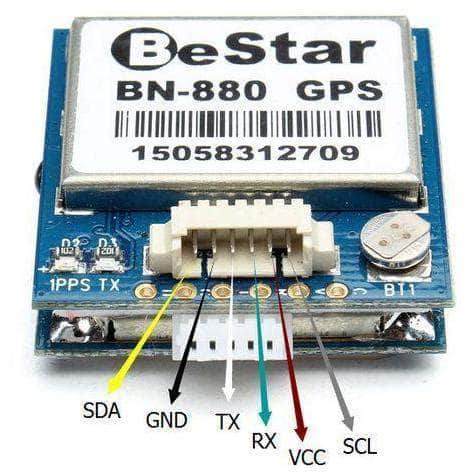
\includegraphics[width=0.4\textwidth]{Imagenes/Bitmap/bn-880}
        \caption{GPS bn-880}
        \label{fig:bn-880}
    \end{figure}
    \item \textbf{Cámara:} se utiliza el modelo oficial de la Raspberry Pi~\cite{raspiCamV2} con interfaz CSI. Permite la captura de vídeo codificado en H.264 mediante la GPU, sin comprometer el rendimiento del sistema.
    \begin{figure}[h]
        \centering
        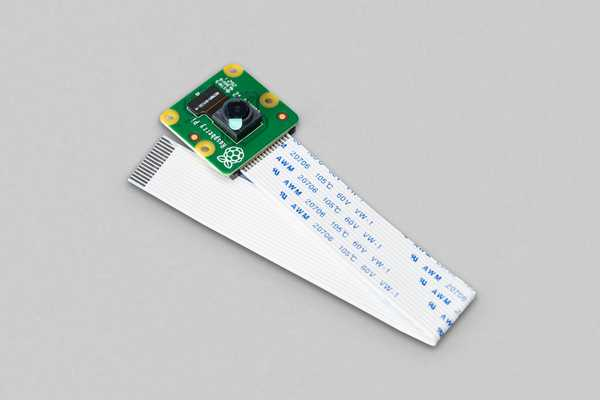
\includegraphics[width=0.4\textwidth]{Imagenes/Bitmap/rascamv2}
        \caption{Raspberry Pi Camera Module 2}
        \label{fig:rascamv2}
    \end{figure}
    \item \textbf{Transmisión de datos:} el sistema utiliza Wi-Fi si hay red disponible, en caso contrario el módulo LoRa E32-900T20D~\cite{ebyteE32}.
    Este módulo opera en 868~MHz y permite comunicación a larga distancia mediante UART.
    \begin{figure}[h]
        \centering
        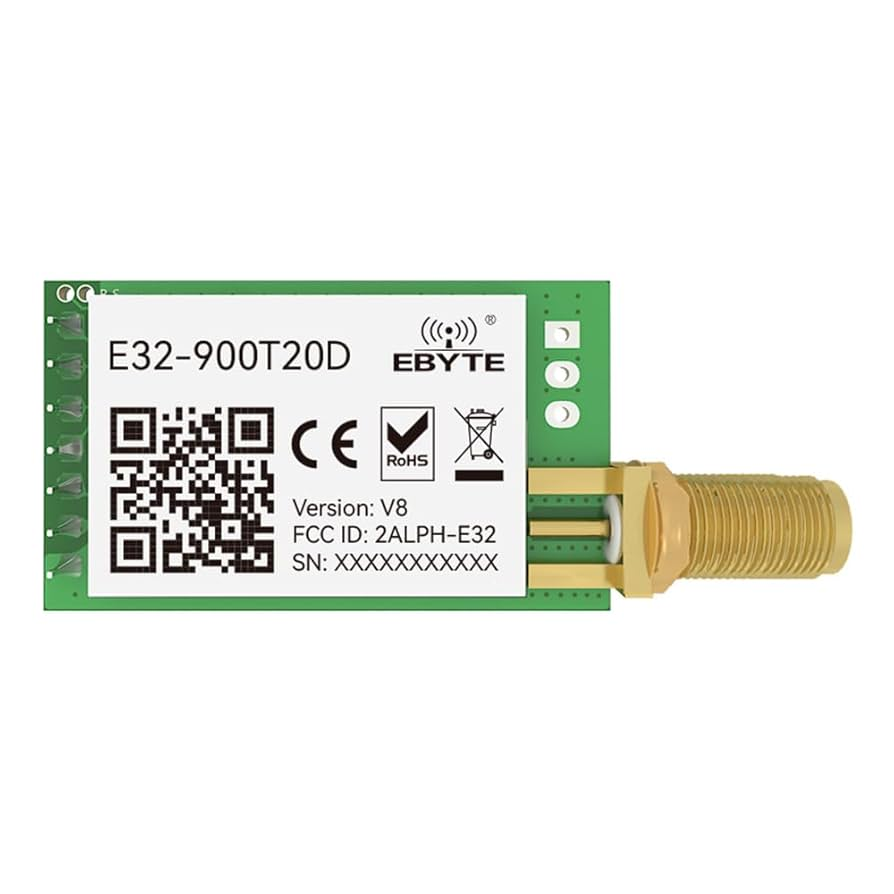
\includegraphics[width=0.4\textwidth]{Imagenes/Bitmap/lorae32}
        \caption{Módulo LoRa E32-900T20D}
        \label{fig:lorae32}
    \end{figure}

    \item \textbf{Alimentación:} el sistema se alimenta mediante una batería recargable de ion de litio (Li-ion) tipo 18650 de 3{,}7~V conectada a un cargador MCP73871~\cite{mcp73871Datasheet}, que permite la recarga mediante panel solar y proporciona protección frente a sobrecarga, descarga profunda y cortocircuitos.

    Para obtener los 5~V requeridos por la Raspberry Pi, se emplea un convertidor elevador DC-DC ajustable (modelo VISSQH), que incrementa la tensión de entrada hasta una salida estabilizada.

    \begin{figure}[H]
        \centering
        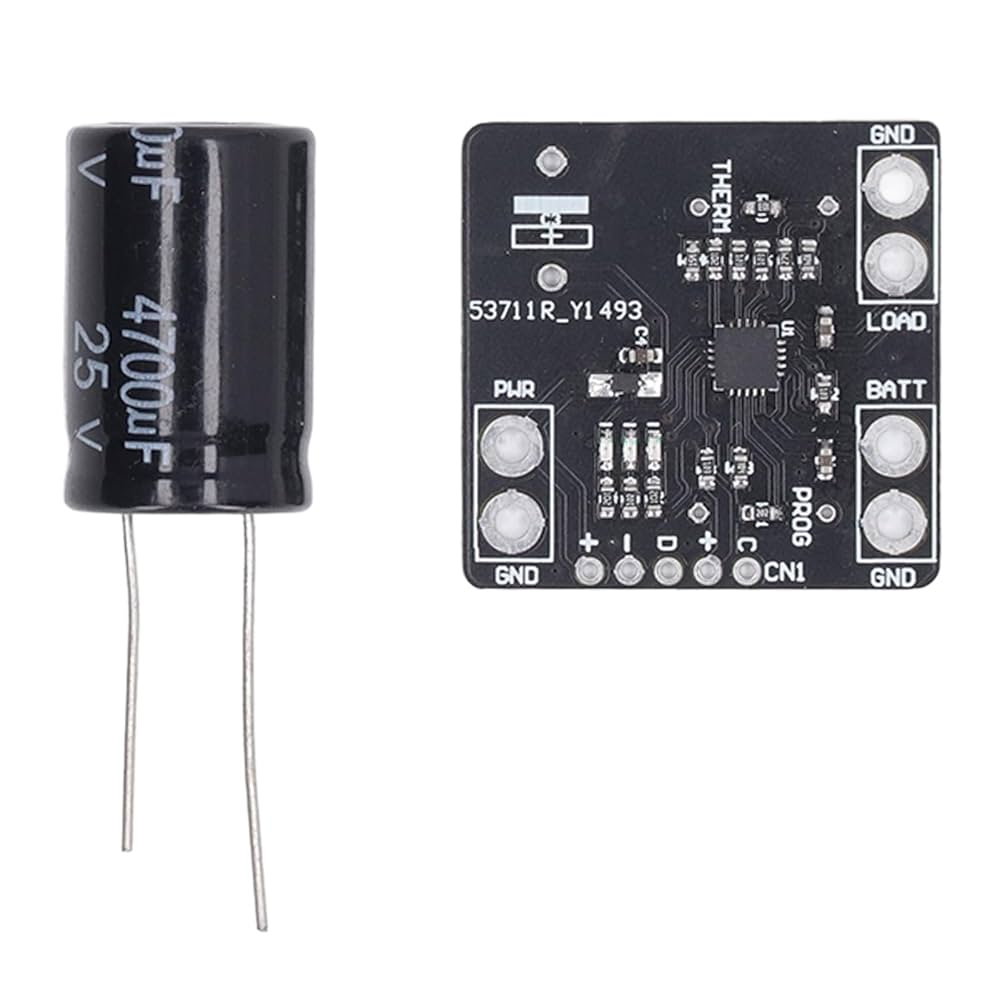
\includegraphics[width=0.4\textwidth]{Imagenes/Bitmap/mcp73871}
        \caption{Cargador MCP73871}
        \label{fig:mcp73871}
    \end{figure}
    \begin{figure}[H]
        \centering
        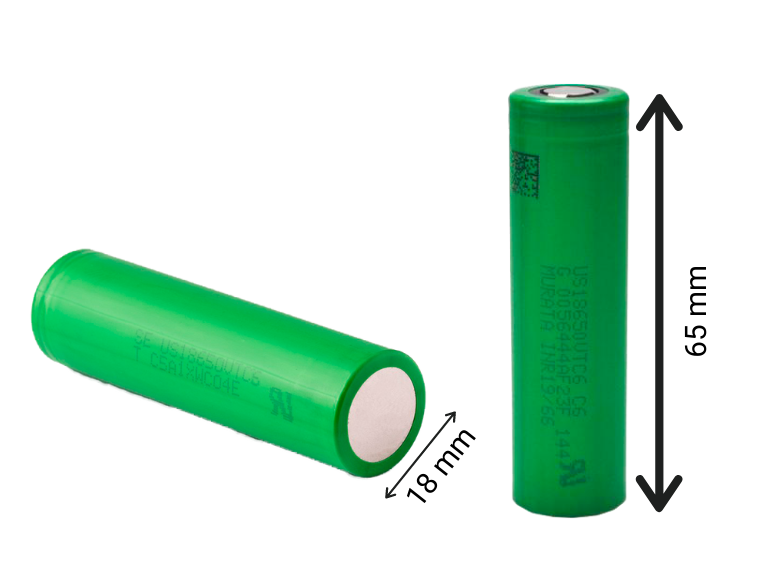
\includegraphics[width=0.4\textwidth]{Imagenes/Bitmap/18650}
        \caption{Batería 18650}
        \label{fig:18650}
    \end{figure}
    \item \textbf{Estación de tierra:} está formada por un receptor LoRa conectado mediante UART a una Raspberry Pi 4.

    Esta actúa como pasarela entre el CanSat y el sistema de mensajería RabbitMQ, reenviando los datos recibidos a través de LoRa.

    \item \textbf{Software embebido:} tanto la Raspberry Pi usada en el CanSat como la de la estación de tierra ejecutan scripts desarrollados en Python.

    \item \textbf{Software del sistema:} el backend está desarrollado en Java utilizando el framework Spring Boot, que facilita la construcción de servicios web REST y la integración con sistemas de mensajería.

    Para el intercambio de mensajes se emplea RabbitMQ, un sistema de colas que implementa el protocolo AMQP.

    La persistencia de datos se gestiona con PostgreSQL, un sistema de gestión de bases de datos relacional.

    La interfaz de usuario está implementada en Flutter, un framework multiplataforma desarrollado en Dart, y establece la comunicación en tiempo real mediante WebSocket utilizando el protocolo STOMP.
\end{itemize}


\section{Arquitectura general del sistema}


\section{Montaje electrónico del CanSat}


\section{Código embebido en la Raspberry Pi}


\section{Backend con Spring Boot}


\section{Frontend con Flutter para visualización en tiempo real}


\section{Pruebas de integración y validación}

